\section{Ejercicio 3}

En este ejercicio nos dan una matriz de sueldos correspondientes a cada posible cargo y antigüedad que puede tener un docente. A partir del cargo y antigüedad de un docente, lo que cobra es equivalente a $\sum_{i = 1}^{cargo} \sum_{j = 1}^{antiguedad} sueldos[i][j]$. Ahora bien un docente siempre tiene aspiraciones más altas con lo cual a pesar de tener un cargo c$_1$ y una antigüedad a$_1$, en realidad aspira a tener cargo c$_2$ y antigüedad a$_2$. \newline

Lo que le interesa saber es el monto de lo que cobraría si tuviera cargo c$_2$ y antigüedad a$_2$, que no podría conseguir si mantuviera su cargo c$_1$ (pudiendo aumentar su antigüedad hasta a$_2$) o si bien mantuviera su antigüedad (pudiendo subir de cargo hasta c$_2$). Vamos a asumir que a$_2$ y c$_2$ siempre son mayores o iguales a a$_1$ y c$_1$ respectivamente, la antigüedad de por sí no puede bajar, y no tiene demasiado sentido que un docente aspire a tener un peor cargo. \newline

Es decir, lo que nos interesa calcular es $\sum_{i = 1}^{c_2} \sum_{j = 1}^{a_2} sueldos[i][j]$ menos lo que gana actualmente y lo que podría ganar si mantiene fijo el cargo y sube su antigüedad o si mantiene fijo la antigüedad y sube el cargo (sin pasarse de c$_2$ ni de a$_2$). En términos de la matriz de sueldos, tenemos: 

\begin{enumerate}
	\item Lo que ganaría con cargo c$_2$ y antigüedad a$_2$ : $\sum_{i = 1}^{c_2} \sum_{j = 1}^{a_2} sueldos[i][j]$
	\item Lo que gana actualmente con cargo c$_1$ y antigüedad a$_1$ : $\sum_{i = 1}^{c_1} \sum_{j = 1}^{a_1} sueldos[i][j]$
	\item Lo que puede ganar como máximo manteniendo cargo c$_1$ pero subiendo antigüedad : $\sum_{i = 1}^{c_1} \sum_{j = 1}^{a_2} sueldos[i][j]$
	\item Lo que puede ganar como máximo manteniendo antigüedad a$_1$ pero subiendo cargo : $\sum_{i = 1}^{c_2} \sum_{j = 1}^{a_1} sueldos[i][j]$
\end{enumerate}

En definitiva, lo que queremos es la primera $-$ la unión de las otras 3. El problema por un lado es que la tercera y cuarta incluyen a la segunda ($a_2 \geq a_1\ y\ c_2 \geq c_1$) y por otro, la intersección de la tercera y la cuarta es efectivamente la segunda. Con lo cual no podemos realizar la resta de una, ya que estaríamos restando algunos sueldos múltiples veces. Hay varias formas de resolver esto. \newline

Una de ellas sería hacer que cada conjunto sea independiente, para que no haya posibilidad de estar restando lo mismo múltiples veces. Esto sería hacer $\sum_{i = 1}^{c_2} \sum_{j = 1}^{a_2} sueldos[i][j]$ - $\sum_{i = 1}^{c_1} \sum_{j = 1}^{a_1} sueldos[i][j]$ - $\sum_{i = c_1}^{c_1} \sum_{j = a_1 + 1}^{a_2} sueldos[i][j]$ - $\sum_{i = c_1 + 1}^{c_2} \sum_{j = a_1}^{a_1} sueldos[i][j]$. La nombraremos la forma complicada.  \newline

Otra forma sería sumar lo que se repite, como para cancelar lo que resté múltiples veces. Esto sería hacer $\sum_{i = 1}^{c_2} \sum_{j = 1}^{a_2} sueldos[i][j]$ - $\sum_{i = 1}^{c_1} \sum_{j = 1}^{a_2} sueldos[i][j]$ - $\sum_{i = 1}^{c_2} \sum_{j = 1}^{a_1} sueldos[i][j]$ + $\sum_{i = 1}^{c_1} \sum_{j = 1}^{a_1} sueldos[i][j]$. La nombraremos la forma copada.  \newline

Otra forma sería calcular directamente lo que queremos, que es $\sum_{i = c_1 + 1}^{c_2} \sum_{j = a_1 + 1}^{a_2} sueldos[i][j]$. La nombraremos la forma ineficiente.

\subsection{Resolviendo el problema}

En definitiva, una posible solución es por cada una de las sumatorias que necesito, recorrer la matriz y sumar lo que necesito. Luego es cuestión de aplicar alguna de las cuentas mencionadas. El problema de esto es que la complejidad depende en el mejor de los casos (forma ineficiente) de $(c_2 - c_1) \times (a_2 - a_1)$. El sólo hecho de leer el input para guardar la matriz nos da $O(a \times c)$, mientras que la complejidad que nos piden es $O(a \times c + q)$. Si por cada pregunta calculamos la respuesta en $O((c_2 - c_1) \times (a_2 - a_1))$, no nos daría la complejidad requerida.  \newline

Lo que vamos a buscar hacer es resolver cada pregunta en O(1). Para hacer esto, en vez de guardarnos la matriz de los sueldos, en la posición (i, j) vamos a guardarnos la sumatoria de los sueldos con cargo menor o igual a i y antigüedad menor o igual a j. Es decir, $\sum_{i = 1}^{i} \sum_{j = 1}^{j} sueldos[i][j]$. Si pudiésemos realizar esto en $O(a \times c)$, podríamos usar la forma complicada y tener tanto $\sum_{i = 1}^{c_2} \sum_{j = 1}^{a_2} sueldos[i][j]$ como $\sum_{i = 1}^{c_1} \sum_{j = 1}^{a_1} sueldos[i][j]$ en O(1), mientras que $\sum_{i = c_1}^{c_1} \sum_{j = a_1 + 1}^{a_2} sueldos[i][j]$ y $\sum_{i = c_1 + 1}^{c_2} \sum_{j = a_1}^{a_1} sueldos[i][j]$ lo podría calcular recorriendo la matriz original en $O((c_2 - c_1) + (a_2 - a_1))$.  \newline

Pero queremos O(1). Podríamos ver cómo calcular las 2 otras partes en O(1), o bien usar la forma copada que son todas cuentas con ambos índices empezando en 1, que son datos que tengo en mi matriz. $\sum_{i = 1}^{c_2} \sum_{j = 1}^{a_2} sueldos[i][j]$ es equivalente a mi nueva matriz en la posición (c$_2$, a$_2$), $\sum_{i = 1}^{c_1} \sum_{j = 1}^{a_2} sueldos[i][j]$ en la posición (c$_1$, a$_2$), $\sum_{i = 1}^{c_2} \sum_{j = 1}^{a_1} sueldos[i][j]$ en la posición (c$_2$, a$_1$) y $\sum_{i = 1}^{c_1} \sum_{j = 1}^{a_1} sueldos[i][j]$ en la posición (c$_1$, a$_1$). Es decir, accediendo a la matriz en O(1), podría hacer esas 3 cuentas (1 sumas y 2 restas) en O(1) y así cumplir con lo requerido.  \newline

Resta ver entonces cómo formar la matriz que quiero de las sumatorias en $O(a \times c)$. Para hacer esto, lo que vamos a hacer es ir recorriendo la matriz original en orden izquierda a derecha, abajo hacia arriba. Es decir, nos movemos por las columnas y al llegar a la última, avanzamos de fila y volvemos a empezar con las columnas. Veamos que si quiero calcular lo que debo poner en (i, j), eso es equivalente a lo que había en la matriz original en (i, j) + la matriz en (i, j - 1) + la matriz en (i - 1, j) - la matriz en (i - 1, j - 1).  \newline

Por el orden en que voy calculando, lo que hay arriba y a la izquierda ya lo tengo calculado, con lo cual tengo la información que necesito ya calculada. Veamos por ejemplo que queremos calcular la posición (4, 4).

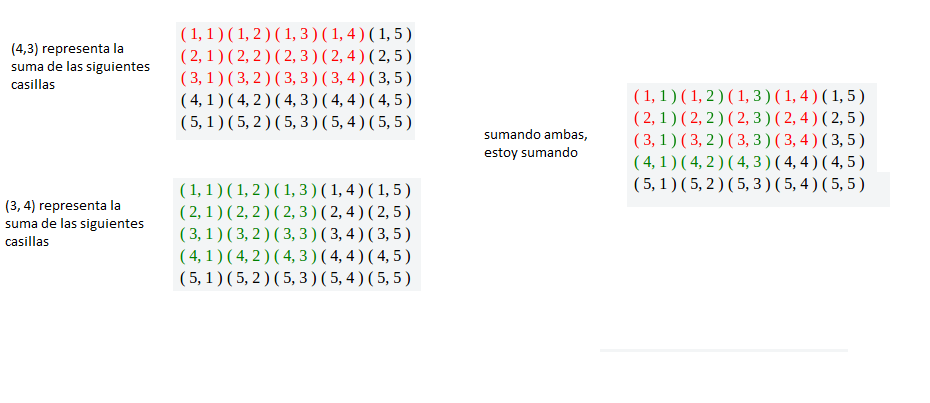
\includegraphics[scale=0.5]{img/tabla.jpg}

Como puede verse en el dibujo, si sumo lo que hay en la matriz en (i, j - 1) + lo que hay en la matriz en (i - 1, j), estoy sumando la intersección 2 veces. Esta intersección corresponde a lo que hay en la matriz en (i - 1, j - 1). Con lo cual si hago M(i, j - 1) + M(i - 1, j) - M(i - 1, j - 1), estoy sumando cada parte 1 sola vez, y luego sólo resta sumarle el valor del sueldo en la matriz original en la posición (i, j) para tener lo que quería : la sumatoria de lo que hay arriba y a la izquierda, incluyendo (i, j). \newline

Una vez obtenida esta matriz, puedo resolver cada pregunta en O(1), basta con hacer la cuenta mencionada en la forma copada. Como cada pregunta la resolvemos en O(1) y hay q preguntas, y como para armar la matriz simplemente hago 4 accesos a matriz, 2 sumas y 1 resta por cada posición, es O(1) para calcular cada posición y hay $a \times c$ posiciones, con lo cual la complejidad de resolver el problema me queda O ($a \times c + q$), cumpliendo con lo pedido.

\subsection {Detalles de implementación}

Como para calcular una posición de la matriz accedo a (i, j - 1),  (i - 1, j) y (i - 1, j - 1), es posible que en los casos borde (los bordes de arriba y a la izquierda de la matriz) alguna de estas posiciones no exista. Con lo cual, habría que hacer las sumas y restas correspondientes sólo si existen esas posiciones en la matriz. Para evitar estos chequeos, lo que hacemos es en vez de tener una matriz de $a \times c$, tenemos una matriz de $(a + 1) \times (c + 1)$ (que no modifica la complejidad) como para que nos \"sobre\" los bordes de arriba y a la izquierda. \newline

En estos bordes colocamos todos 0, así después cuando haga las cuentas estas posiciones siempre existen y sumar o restar 0 si no había nada, es justamente lo que quería, el 0 es el elemento neutro de la suma y resta así que nos sirve para lo que queremos. Además de esta manera no tenemos que preocuparnos por que la matriz sea 0-indexed y las coordenadas que nos dan (cargo y antigüedad) con las preguntas son 1-indexed. De esta forma, no hay que estar restando 1 a las coordenadas que nos dan para pasarlo a 0-indexed.\newline

Otro detalle es que la matriz de las sumatorias se puede ir calculando a medida que leo el input, ya que el orden en que decidí calcular la matriz es el mismo orden en que leo el input. Sólo hay que tener cuidado de iniciar la primer fila y primer columna con 0 antes de leer el input para los casos borde mencionados. \newline

Hay que mencionar también que estamos suponiendo en la implementación que la suma de todos los sueldos no se pasa de lo que puede almacenar un int, de no ser así habría que usar long o lo necesario para que no suceda. Estamos suponiendo también que a$_2$ y c$_2$ son $\geq$ a$_1$ y c$_1$ respectivamente ya que entendimos que en este problema eso es lo más lógico.

\subsection {Pseudocódigo}

\begin{algorithmic}

	\State $matriz[cargos + 1][antiguedad + 1] \gets [0...0]$ \Comment{Inicializo una matriz con ceros por lo menos en la primer fila y primer columna}

	\For{c $\gets$ 1 .. cargos}
		\For{a $\gets$ 1 .. antigüedad}
			\State $matriz[c][a] \gets leer\_input()$
			\State $matriz[c][a] \gets matriz[c][a] + matriz[c - 1][a] + matriz[c][a - 1] + matriz[c - 1][a - 1]$
		\EndFor
	\EndFor

	\For{q $\gets$ 1 .. preguntas}
		\State $c_1, a_1, c_2, a_2 \gets leer\_input()$
		\State $res \gets matriz[c_2][a_2] - matriz[c_2][a_1] - matriz[c_1][a_2] + matriz[c_1][a_1]$
		\State mostrar(res)
	\EndFor

\end{algorithmic}